%
% Copyright (c) 2017 Intel Corporation
%
% Permission is hereby granted, free of charge, to any person obtaining a copy
% of this software and associated documentation files (the "Software"), to
% deal in the Software without restriction, including without limitation the
% rights to use, copy, modify, merge, publish, distribute, sublicense, and/or
% sell copies of the Software, and to permit persons to whom the Software is
% furnished to do so, subject to the following conditions:
%
% The above copyright notice and this permission notice shall be included in
% all copies or substantial portions of the Software.
%
% THE SOFTWARE IS PROVIDED "AS IS", WITHOUT WARRANTY OF ANY KIND, EXPRESS OR
% IMPLIED, INCLUDING BUT NOT LIMITED TO THE WARRANTIES OF MERCHANTABILITY,
% FITNESS FOR A PARTICULAR PURPOSE AND NONINFRINGEMENT. IN NO EVENT SHALL THE
% AUTHORS OR COPYRIGHT HOLDERS BE LIABLE FOR ANY CLAIM, DAMAGES OR OTHER
% LIABILITY, WHETHER IN AN ACTION OF CONTRACT, TORT OR OTHERWISE, ARISING
% FROM, OUT OF OR IN CONNECTION WITH THE SOFTWARE OR THE USE OR OTHER DEALINGS
% IN THE SOFTWARE.
%

\newcommand{\repoTopPath}{../../..}
\newcommand{\commonPreamblePath}{\repoTopPath/common/latex/common_preamble.tex}
\input \commonPreamblePath

%----BEGIN TYPESETTING----------------------------------------------------------
\begin{document}
\sffamily

% create our own title area rather than \begin{titlepage} or \maketitle
\begin{center}
\let\savethefootnote\thefootnote
\let\thefootnote\relax\footnote{Intel, and Quartus are trademarks of Intel Corporation or its subsidiaries in the U.S. and/or other countries.}
\addtocounter{footnote}{-1}
\let\thefootnote\savethefootnote
\hspace{-1em}
\let\savethefootnote\thefootnote
\let\thefootnote\relax\footnote{Other names and brands may be claimed as the property of others.}
\addtocounter{footnote}{-1}
\let\thefootnote\savethefootnote
\hspace{-1em}
\LARGE{My First Qsys System}\\[1em]
\end{center}

\begin{flushleft}
\normalsize{PDF created: \today}\\
\normalsize{Validated using tools release: \TheToolsReleaseVersion}
\end{flushleft}

% make an entry in the PDF bookmarks for the TOC
\pdfbookmark[0]{Contents}{sumario_label}
% insert the default TOC format
\tableofcontents

%----NEW SECTION DEFINITION-----------------------------------------------------
\section*{Overview}
% must manually add TOC reference for unnumbered section
\addcontentsline{toc}{section}{Overview}
%----NEW SECTION DEFINITION-----------------------------------------------------

\begin{flushleft}
\noindent
This tutorial demonstrates how to use the Qsys tool to easily create an FPGA design using IP available in the Intel\textsuperscript{\textregistered} Quartus\textsuperscript{\textregistered} software IP catalog.  Qsys speeds embedded system design by standardizing the interconnect between IP blocks and allowing users to create their own IP blocks for reuse in their systems.

\end{flushleft}

%----NEW SECTION DEFINITION-----------------------------------------------------
\section*{Prerequisites}
% must manually add TOC reference for unnumbered section
\addcontentsline{toc}{section}{Prerequisites}
%----NEW SECTION DEFINITION-----------------------------------------------------

\begin{flushleft}
\noindent
The following are required:

\begin{itemize}

\item Windows\textsuperscript{*} or Linux\textsuperscript{*} development host PC

\item Installed Intel Quartus Prime Software.  Either the Lite or Standard Edition, but not the Pro Edition.
\item Completed Intel Quartus software project from \textquote{How to Program Your First FPGA Device}
\begin{itemize}
\item Either follow the tutorial steps presented \href{\TheReleasesURL/writeup_MyFirstFPGA.pdf}{\underline{here}}.
%\item Or, you can extract this PDF attachment to your local file system: \textattachfile[
%	color=0.0 0.678 0.937,
%	mimetype=application/zip,
%	description={ZIP Archvie File: blink.zip}
%]{../blink_archive/blink.zip}{\textbf{blink.zip}}. Right click on the PDF attachment link and your PDF reader should present a pop-up menu with an option to save the attachment to your local file system.
\item Or, you can download an archive of the required contents from that tutorial to your local file system \href{\TheReleasesURL/blink_for_MyFirstQsysSystem.zip}{\underline{here}}.
\end{itemize}

\end{itemize}

\begin{tcolorbox}[
	colback=MyMintedBGColor,
	colframe=MyMintedBGColor,
	]

\textbf{Note:} User experience may vary when using earlier or later versions of Intel Quartus software.  Screenshots in this document are based on the 17.0 release.

\end{tcolorbox}

\end{flushleft}

\newpage

%----NEW SECTION DEFINITION-----------------------------------------------------
\section*{Creating the Qsys System}
% must manually add TOC reference for unnumbered section
\addcontentsline{toc}{section}{Creating the Qsys System}
%----NEW SECTION DEFINITION-----------------------------------------------------

\begin{flushleft}
\noindent

This section will describe the steps required to create a Qsys system.  It assumes that you have the completed \textbf{blink} Intel Quartus software project from the \textquote{How to Program Your First FPGA Device} tutorial open.

\begin{enumerate}[
	label=\textbf{Step \arabic*.},
	leftmargin=*,
	widest={00},
	align=left]

\item With the \textbf{blink} Intel Quartus software project from the previous tutorial open in the tool, start by launching Qsys by clicking the Qsys button on the toolbar, or select Qsys from the \textbf{Tools} menu.

\begin{figure}[H]
\centering
% screen shots report a density of 37.8 PixelsPerCentimeter when actual resolution
% is more like 56 PixelsPerCentimeter, so the scaling factor for 1:1 is 0.675
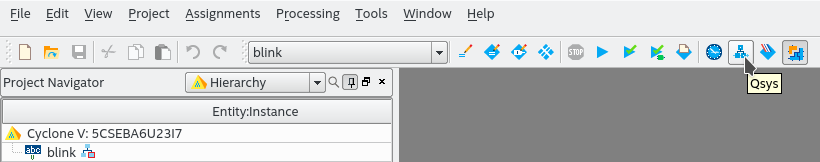
\includegraphics[scale=0.675]{01-qsys-button}
\caption{Qsys Button on Intel Quartus Software Toolbar}
\label{fig:01-qsys-button}
\end{figure}

\begin{figure}[H]
\centering
% screen shots report a density of 37.8 PixelsPerCentimeter when actual resolution
% is more like 56 PixelsPerCentimeter, so the scaling factor for 1:1 is 0.675
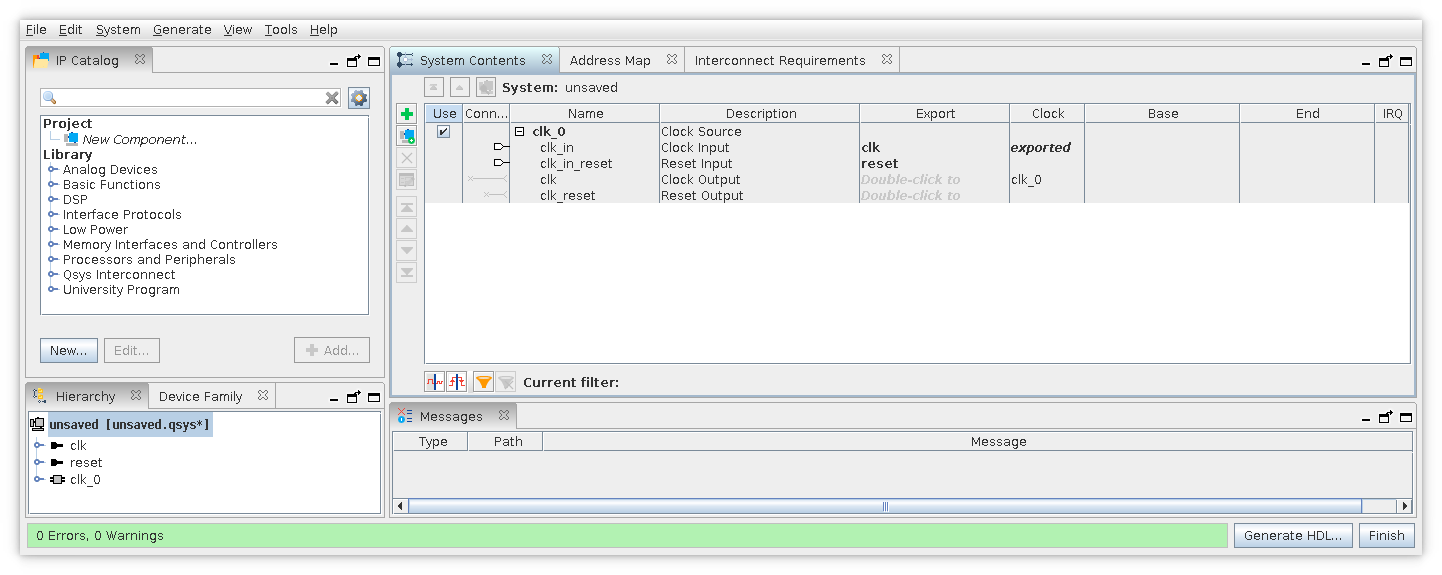
\includegraphics[scale=0.475]{01-qsys-open}
\caption{New Empty Qsys System}
\label{fig:01-qsys-open}
\end{figure}

\newpage

\item Qsys opens to an unsaved system, with one clock source component already instantiated.  To add another IP block, use the \textbf{IP Catalog} pane in the left hand column.  In the search bar, start typing \textbf{on-chip memory} until you see the \textbf{On-Chip Memory (RAM or ROM)} IP appear.

\begin{figure}[H]
\centering
% screen shots report a density of 37.8 PixelsPerCentimeter when actual resolution
% is more like 56 PixelsPerCentimeter, so the scaling factor for 1:1 is 0.675
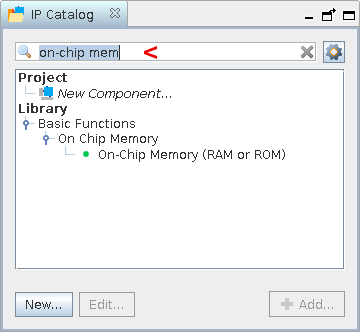
\includegraphics[scale=0.675]{02-ocmem-search}
\caption{Search for On-Chip Memory Component}
\label{fig:02-ocmem-search}
\end{figure}

\newpage

\item Either double click on the On-Chip Memory component or select it with the mouse and click the \textbf{Add...} button to insert a new instance into the system.  This opens the parameter dialog for the On-Chip Memory IP.  Change the \textbf{Slave S1 Data Width} to \textbf{64}, and change the \textbf{Total Memory Size} field to \textbf{65536} to make this a 64-kilobyte on-chip memory that supports 64-bit data accesses, then click the \textbf{Finish} button at the bottom right of the dialog box.

\begin{figure}[H]
\centering
% screen shots report a density of 37.8 PixelsPerCentimeter when actual resolution
% is more like 56 PixelsPerCentimeter, so the scaling factor for 1:1 is 0.675
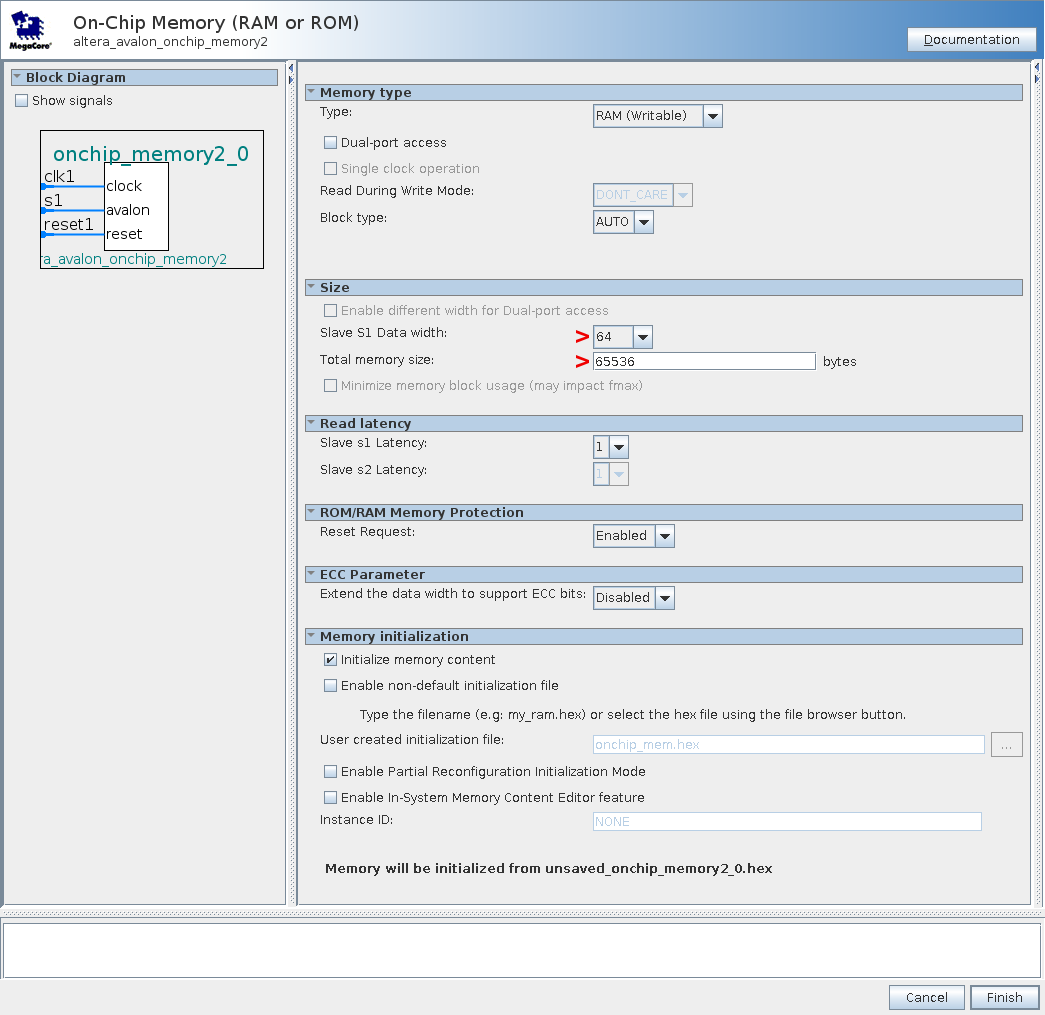
\includegraphics[scale=0.600]{03-ocmem-parameters}
\caption{On-Chip Memory Parameters Dialog}
\label{fig:03-ocmem-parameters}
\end{figure}

\newpage

\item With the new memory component instantiated in the system, we should give it a more meaningful name to us.  To rename components in Qsys, select the component then right click to bring up the context pop-up menu, and select \textbf{Rename}.  Rename the on-chip memory from \textbf{onchip\_memory2\_0} to \textbf{ocram\_64k}.

\begin{figure}[H]
\centering
% screen shots report a density of 37.8 PixelsPerCentimeter when actual resolution
% is more like 56 PixelsPerCentimeter, so the scaling factor for 1:1 is 0.675
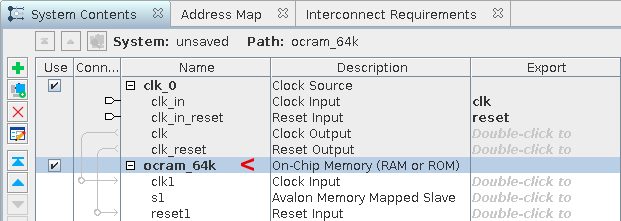
\includegraphics[scale=0.675]{04-ocram-rename}
\caption{Renamed On-Chip Memory Component}
\label{fig:04-ocram-rename}
\end{figure}

\item To connect components in Qsys, use the \textbf{Connections} column in the \textbf{System Contents} pane.  Possible connections of similar types are presented as circles at the intersection points and shaded in gray.  They become active connections when the circle is clicked and turns black.  First, connect the \textbf{clk\_0} clock output with the \textbf{ocram\_64k} clock input.  Then, connect the \textbf{clk\_0} reset output with the \textbf{ocram\_64k} reset input.   The system should now look like the image below.

\begin{figure}[H]
\centering
% screen shots report a density of 37.8 PixelsPerCentimeter when actual resolution
% is more like 56 PixelsPerCentimeter, so the scaling factor for 1:1 is 0.675
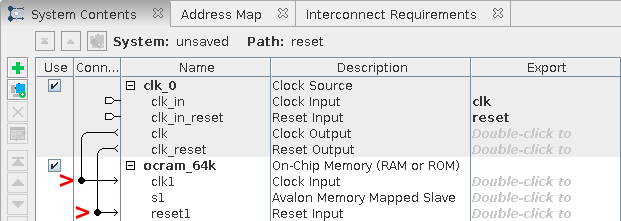
\includegraphics[scale=0.675]{05-clk-ocram-connected}
\caption{Clock and Reset Connections to On-Chip Memory}
\label{fig:05-clk-ocram-connected}
\end{figure}

Notice how the Avalon Memory Mapped Slave connection on the on-chip RAM does not yet have an available connection.  That connection will not appear until an IP with a matching Avalon Memory Mapped Master is added, which will be done in a later step.

\newpage

Also note that hovering the mouse over a connection point brings up a tool tip that details the interfaces to be connected.  This can be useful while building larger systems.

\begin{figure}[H]
\centering
% screen shots report a density of 37.8 PixelsPerCentimeter when actual resolution
% is more like 56 PixelsPerCentimeter, so the scaling factor for 1:1 is 0.675
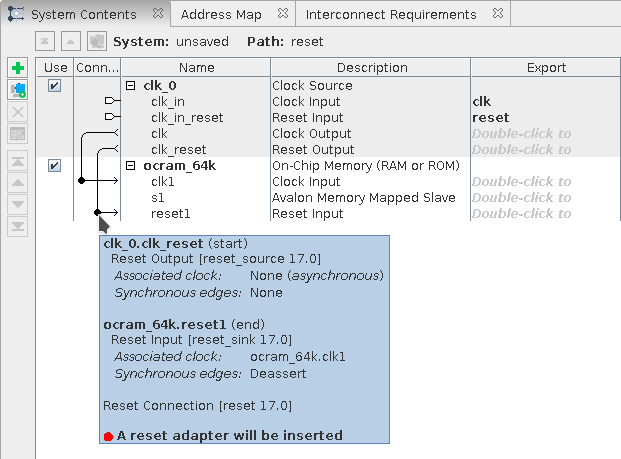
\includegraphics[scale=0.675]{05-clk-ocram-rst-tooltip}
\caption{Connection Point Tooltip Pop-ups}
\label{fig:05-clk-ocram-rst-tooltip}
\end{figure}

\item Adding further IP follows the same process.  To complete the system, add the following IP, and connect the clock and reset interfaces for each.

\begin{enumerate}[
	label=\textbf{Step \arabic{enumi}\alph*.},
	leftmargin=*,
	align=left]

\item Add a second, small \textbf{On-Chip Memory (RAM or ROM)}, with 32-bit data width and 16 byte memory size.  The importance of this seemingly redundant component will be explained in a later step.  Rename this component to \textbf{default\_16b}.

\begin{figure}[H]
\centering
% screen shots report a density of 37.8 PixelsPerCentimeter when actual resolution
% is more like 56 PixelsPerCentimeter, so the scaling factor for 1:1 is 0.675
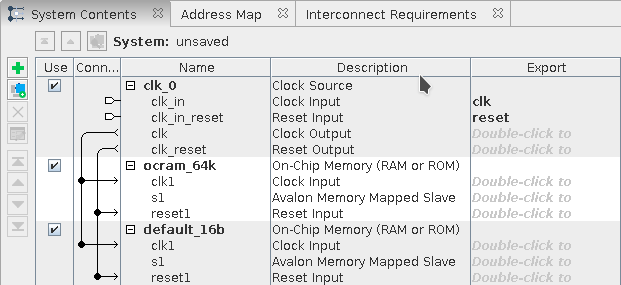
\includegraphics[scale=0.675]{06a-default_16b-ocram-connected}
\caption{default\_16b On-Chip Memory Component}
\label{fig:06a-default_16b-ocram-connected}
\end{figure}

\newpage

\item Add a \textbf{PIO (Parallel I/O)} component with an 8-bit output only.  Rename this component to \textbf{led\_pio}.  Then export the \textbf{external\_connection} interface as \textbf{led\_pio} by double clicking next to the \textbf{external\_connection} interface in the \textbf{Export} column and then edit the default name catenation to just read \textbf{led\_pio}.

\begin{figure}[H]
\centering
% screen shots report a density of 37.8 PixelsPerCentimeter when actual resolution
% is more like 56 PixelsPerCentimeter, so the scaling factor for 1:1 is 0.675
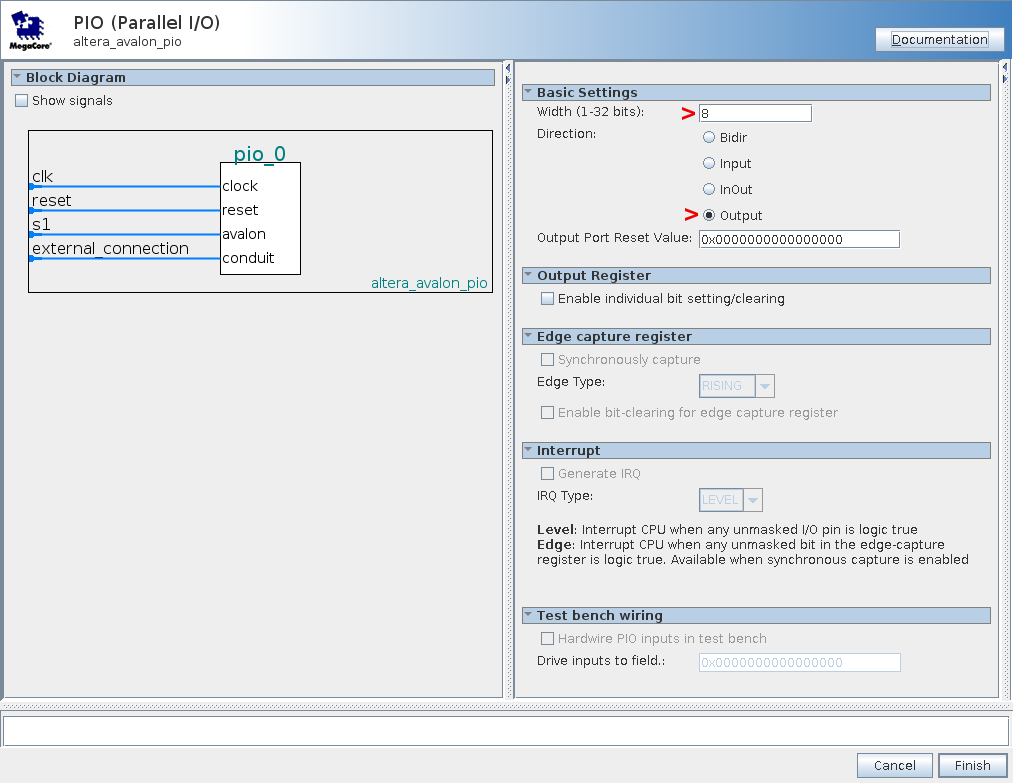
\includegraphics[scale=0.600]{06b-pio-parameters}
\caption{PIO Component Parameters Dialog}
\label{fig:06b-pio-parameters}
\end{figure}

\item Add a PIO component with a 1-bit input only. Rename this component to \textbf{button\_pio} and export the \textbf{external\_connection} interface as \textbf{button\_pio}.

\item Add a PIO component with a 4-bit input only. Rename this component to \textbf{switch\_pio} and export the \textbf{external\_connection} interface as \textbf{switch\_pio}.

\begin{figure}[H]
\centering
% screen shots report a density of 37.8 PixelsPerCentimeter when actual resolution
% is more like 56 PixelsPerCentimeter, so the scaling factor for 1:1 is 0.675
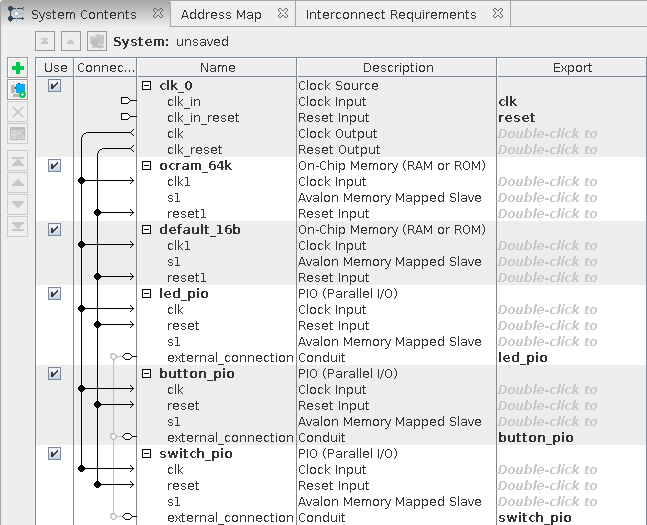
\includegraphics[scale=0.675]{06b-i-pio-connected}
\caption{PIO Components Added to System}
\label{fig:06b-i-pio-connected}
\end{figure}

\item Add a \textbf{System ID} component with a recognizable system ID value. Use \textbf{0xde10de10} as the ID value and rename this component to \textbf{system\_id}.

\begin{figure}[H]
\centering
% screen shots report a density of 37.8 PixelsPerCentimeter when actual resolution
% is more like 56 PixelsPerCentimeter, so the scaling factor for 1:1 is 0.675
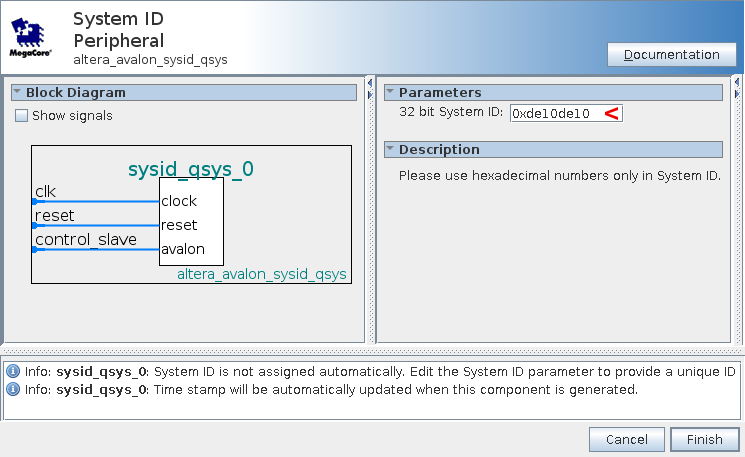
\includegraphics[scale=0.675]{06c-sys-id-parameters}
\caption{System ID Parameters Dialog}
\label{fig:06c-sys-id-parameters}
\end{figure}

\newpage

\item Add a \textbf{JTAG to Avalon Master Bridge}.  Keep the default instance name \textbf{master\_0}.

\begin{figure}[H]
\centering
% screen shots report a density of 37.8 PixelsPerCentimeter when actual resolution
% is more like 56 PixelsPerCentimeter, so the scaling factor for 1:1 is 0.675
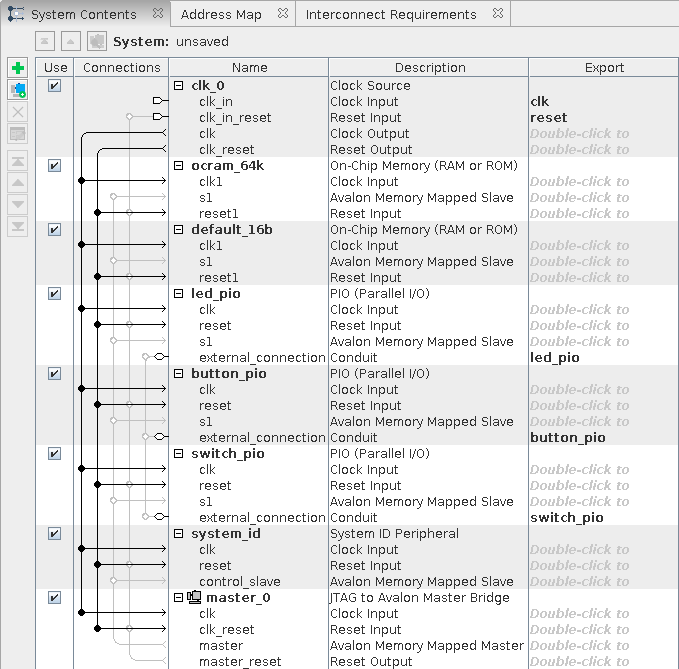
\includegraphics[scale=0.675]{06d-jtag-master-unconnected}
\caption{System ID and JTAG Master Added to System}
\label{fig:06d-jtag-master-unconnected}
\end{figure}

\end{enumerate}

\newpage

\item At this point, the clocks and resets should all be connected, but it was not until the JTAG master bridge was added that any of the other IPs' Avalon Slave interfaces had any connections available.  Now that the JTAG bridge presents an Avalon master, Qsys identifies the similar interfaces and presents the possible connections.  Connect the JTAG bridge master to the other IP slaves, while also connecting the \textbf{master\_reset} reset output to the reset inputs of the other IP blocks.

\begin{figure}[H]
\centering
% screen shots report a density of 37.8 PixelsPerCentimeter when actual resolution
% is more like 56 PixelsPerCentimeter, so the scaling factor for 1:1 is 0.675
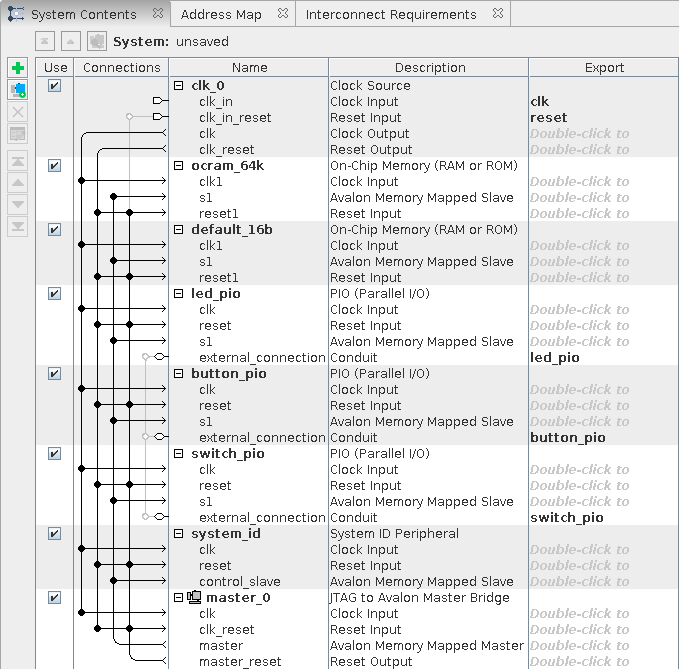
\includegraphics[scale=0.675]{07-jtag-master-avmm-connected}
\caption{Fully Connected System}
\label{fig:07-jtag-master-avmm-connected}
\end{figure}

\item Qsys adds a preliminary address span to each slave, but initially they overlap, creating errors in the \textbf{Messages} pane.

\begin{figure}[H]
\centering
% screen shots report a density of 37.8 PixelsPerCentimeter when actual resolution
% is more like 56 PixelsPerCentimeter, so the scaling factor for 1:1 is 0.675
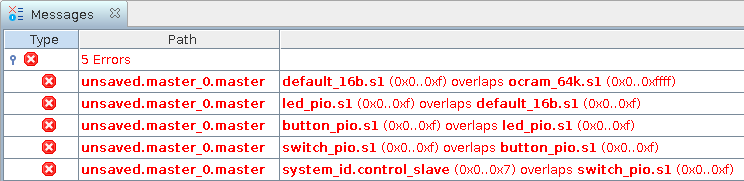
\includegraphics[scale=0.675]{07a-mm-address-conflict-messages}
\caption{Address Span Overlap Errors}
\label{fig:07a-mm-address-conflict-messages}
\end{figure}

To resolve the address span overlap errors, first lock the \textbf{ocram\_64k} On-Chip Memory address range to start at \textbf{0x0000\_0000} by clicking the lock button next to the address in the \textbf{Base} column.  Then, click the \textbf{System} menu, and choose \textbf{Assign Base Addresses}.  Observe the new base addresses for all the IP blocks, and that the address for the On-Chip memory did not change.  In general, \textbf{Assign Base Addresses} will create the most compact address map by packing all of the peripherals in order from largest address span to smallest address span.  There is no guarantee that generated addresses will remain constant over multiple invocations of the \textbf{Assign Base Addresses} command, however locked address spans are not adjusted by the \textbf{Assign Base Addresses} command.  For the simplicity of later tutorials, ensure the base address for each IP matches the below image; they can be edited by double-clicking the address itself.  Finally, right-click any of the column names in the \textbf{System Contents} view, and choose the \textbf{Show Default Slave Column} option.  Scroll to the right, and check the \textbf{Default Slave} box for the \textbf{default\_16b} on-chip memory.

\begin{figure}[H]
\centering
% screen shots report a density of 37.8 PixelsPerCentimeter when actual resolution
% is more like 56 PixelsPerCentimeter, so the scaling factor for 1:1 is 0.675
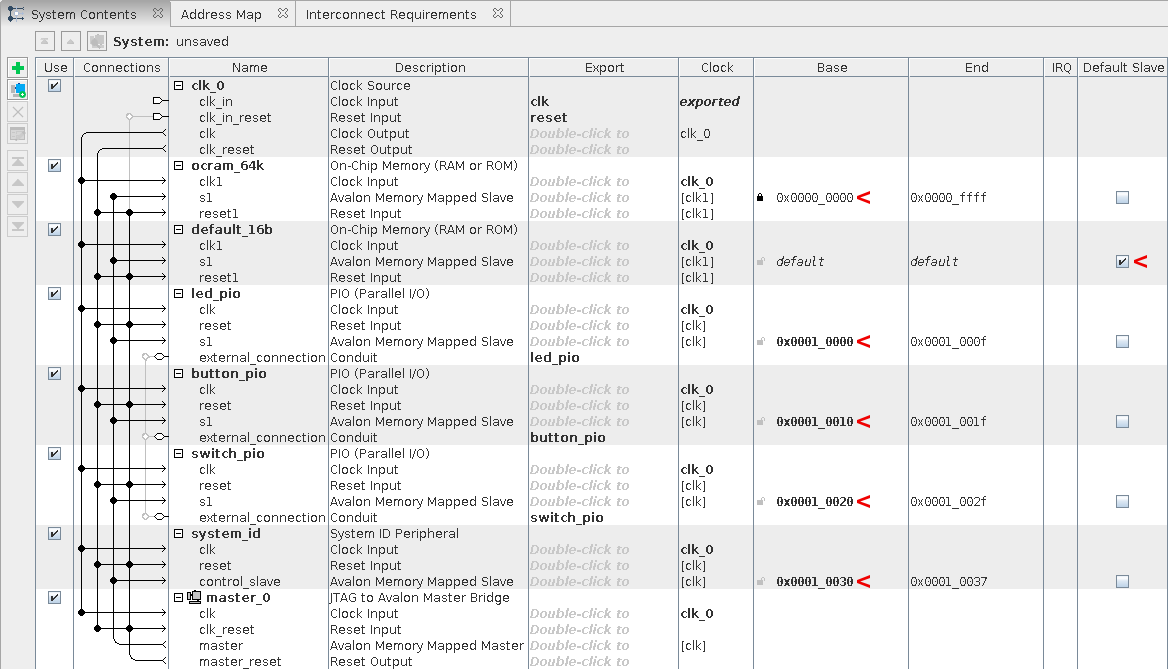
\includegraphics[scale=0.575]{07b-assigned-addresses-default-slave}
\caption{Properly Addressed System}
\label{fig:07b-assigned-addresses-default-slave}
\end{figure}

Default slaves are an important concept.  If a memory mapped read or write transaction is initiated into an unmapped address span, Qsys will route it to the default slave for that master in that interconnect zone.  If you do not specify a default slave, then Qsys chooses by default the peripheral with the largest available address span on that interconnect, which in most cases will be some form of memory since those are typically the largest address span peripherals in a system.  Choosing a default slave allows the designer to explicitly state that all unmapped address accesses should go to that slave.  In this example tutorial, these accesses will be routed to a tiny on-chip memory that is not used for anything else, removing the possibility that data in the main memory or any other peripheral could be corrupted and allowing the designer a space to check whether errant accesses are occurring.

\begin{sloppypar}
If you are interested in seeing a more capable default slave component, checkout the \textbf{trivial\_\allowbreak default\_\allowbreak avalon\_\allowbreak slave} component available in this public GitHub\textsuperscript{*} repository \href{https://github.com/intel/supplemental-reset-components-for-qsys}{https://\allowbreak github.com/\allowbreak intel/\allowbreak supplemental-\allowbreak reset-\allowbreak components-\allowbreak for-\allowbreak qsys}.  That default slave can be parameterized with a variety of responses to errant accesses, like never responding which essentially holds the master in an infinite wait request, reply with a specific data pattern, generate an Avalon error response, generate an interrupt, or generate a reset.
\end{sloppypar}

\newpage

\item The Qsys system is complete, and now it is time to integrate it back into the Intel Quartus software project.  First, save the Qsys system and choose the name \textbf{soc\_system.qsys}.  Close the save window when the save completes.  Then, from the \textbf{Generate} menu, choose \textbf{Generate HDL...}.  This brings up the \textbf{Generate} window, uncheck the \textbf{Create block symbol file (.bsf)} box and click the \textbf{Generate} button.

\begin{figure}[H]
\centering
% screen shots report a density of 37.8 PixelsPerCentimeter when actual resolution
% is more like 56 PixelsPerCentimeter, so the scaling factor for 1:1 is 0.675
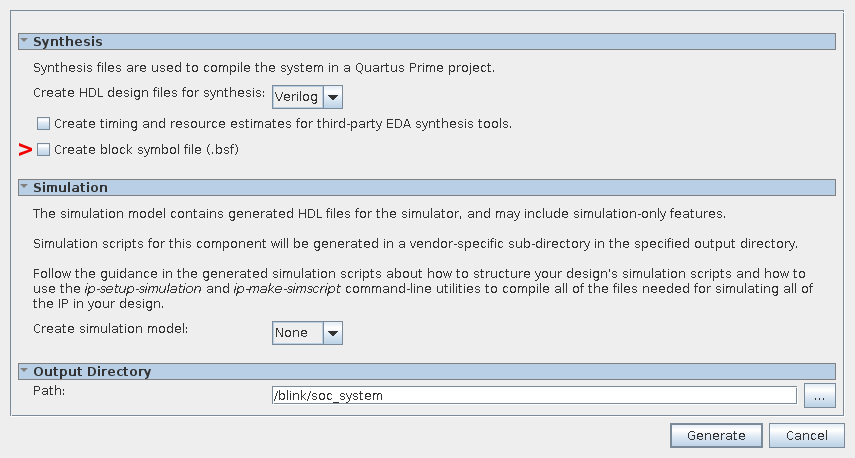
\includegraphics[scale=0.675]{08-generate}
\caption{Qsys Generate Dialog}
\label{fig:08-generate}
\end{figure}

\item Qsys will now generate the HDL files for the IP and interconnect.  Once it finishes, click the \textbf{Close} button, and then click the \textbf{Finish} button at the bottom right of the Qsys window.  This will close Qsys, and present instructions to add the \textbf{.qip} file to the Intel Quartus software project.

\begin{figure}[H]
\centering
% screen shots report a density of 37.8 PixelsPerCentimeter when actual resolution
% is more like 56 PixelsPerCentimeter, so the scaling factor for 1:1 is 0.675
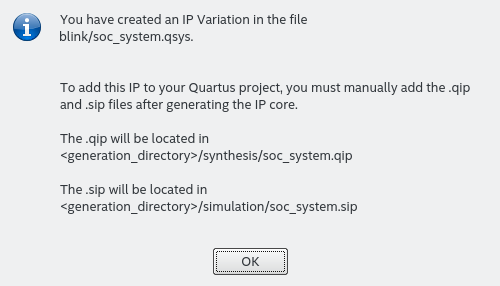
\includegraphics[scale=0.675]{09-qip-window}
\caption{QIP Instruction Dialog}
\label{fig:09-qip-window}
\end{figure}

\end{enumerate}

\end{flushleft}

\newpage

%----NEW SECTION DEFINITION-----------------------------------------------------
\section*{Integrating the Qsys System into the Intel Quartus Software Project}
% must manually add TOC reference for unnumbered section
\addcontentsline{toc}{section}{Integrating the Qsys System into the Intel Quartus Software Project}
%----NEW SECTION DEFINITION-----------------------------------------------------

\begin{flushleft}
\noindent

This section will describe how to incorporate the newly generated Qsys output into the existing \textbf{blink} Intel Quartus software project.

\begin{enumerate}[
	label=\textbf{Step \arabic*.},
	leftmargin=*,
	widest={00},
	align=left]

\item Add the Qsys generated QIP file to the \textbf{blink} project.  Adding the \textbf{.qip} file follows the same process used to add the \textbf{.sdc} file in the prior tutorial.  From the \textbf{Assignments} menu, choose \textbf{Settings} to bring up the \textbf{Settings} window, then select \textbf{Files} on the left \textbf{Category} list.  Click the \textbf{...} button to the right of the \textbf{File Name} box to browse for the file, and navigate to the \textbf{.qip} file using the path described in the dialog when you closed Qsys, select that file and click the \textbf{Open} button to add the file to the project.  Click the \textbf{Apply} button and then click the \textbf{Ok} button to close the settings window.

\begin{figure}[H]
\centering
% screen shots report a density of 37.8 PixelsPerCentimeter when actual resolution
% is more like 56 PixelsPerCentimeter, so the scaling factor for 1:1 is 0.675
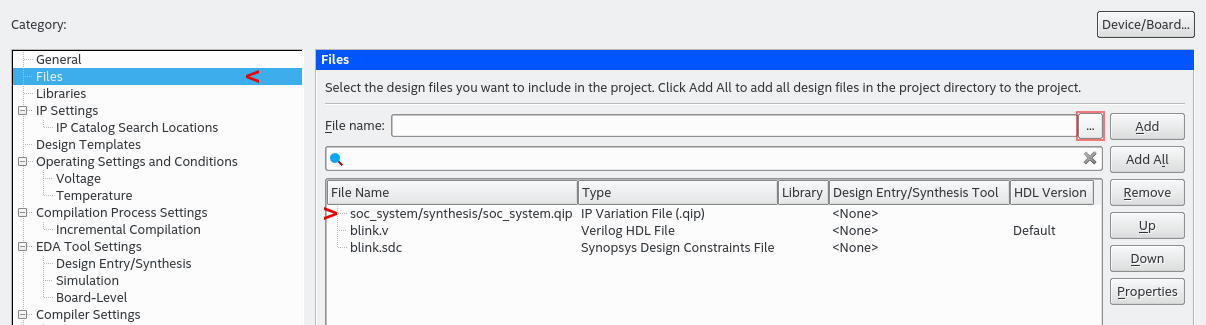
\includegraphics[scale=0.550]{09a-settings-files-qip}
\caption{Adding QIP File to Intel Quartus Software Project}
\label{fig:09a-settings-files-qip}
\end{figure}

\item Qsys creates an instantiation template file for the generated system, in this case it is called \textbf{soc\_\allowbreak system\_\allowbreak inst.v} in the \textbf{soc\_system} folder that is now in the Intel Quartus software project folder.  It is convenient to use this to correctly instantiate the Qsys-generated system in the top-level HDL file.  Replace the existing code in \textbf{blink.v} with the code below:
\newline
\newline
%Extract PDF Attachment: \textattachfile[
%	color=0.0 0.678 0.937,
%	mimetype=text/plain,
%	description={Verilog Source File: blink.v}
%]{../../hdl_src/blink.v}{\textbf{blink.v}}
Download the blink.v file \href{\TheRawURL/MyFirstQsysSystem/hdl_src/blink.v}{\underline{here}}.
\newline
If you wish to view the blink.v file in the GitHub repo you can look \href{\TheBlobURL/MyFirstQsysSystem/hdl_src/blink.v}{\underline{here}}.

\inputminted[
	bgcolor=MyMintedBGColor,
	linenos,
	fontsize=\normalsize
]{verilog}{../../hdl_src/blink.v}

Note the additional instantiated synchronizer in this top level HDL.  When the FPGA is released from configuration mode into user mode, it is done so asynchronously, which can violate design timing constraints and lead to design instability.  The synchronizer provides a brief and stable reset pulse that is synchronously released, allowing the design to cleanly enter operation after power on and configuration. If you are interested in seeing a Qsys component that can provide the power on reset functionality, checkout the \textbf{power\_\allowbreak on\_\allowbreak reset} component available in this public Git repository \href{https://github.com/intel/supplemental-reset-components-for-qsys}{\small{https://\allowbreak github.com/\allowbreak intel/\allowbreak supplemental-reset-components-for-qsys}}.

\item Click the \textbf{Start Analysis \& Elaboration} button on the toolbar to have the Intel Quartus software process the new HDL.  There will be many more messages as the Intel Quartus software processes the Qsys-generated system.  This process will identify any errors in the HDL source files or how they are configured in the project as well as inform the Intel Quartus software of the new top level ports that we declared in our top module.

\begin{figure}[H]
\centering
% screen shots report a density of 37.8 PixelsPerCentimeter when actual resolution
% is more like 56 PixelsPerCentimeter, so the scaling factor for 1:1 is 0.675
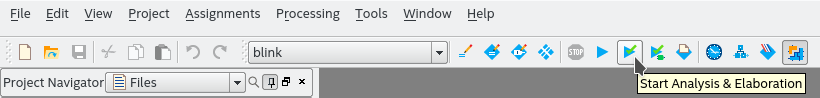
\includegraphics[scale=0.675]{13-quartus-analysis-button}
\caption{Start Analysis and Elaboration Button on Intel Quartus Software Toolbar}
\label{fig:13-quartus-analysis-button}
\end{figure}

\item The new top level module declares many more inputs and outputs than the original design, so new pin constraints will need to be assigned to those inputs and outputs and the stale pin constraints can be removed.  The Terasic DE10-Nano user manual contains the diagrams and schematics where these pin assignments are derived from.  From the \textbf{Assignments} menu, open the \textbf{Pin Planner} tool and assign the pins as in the following image.  The important columns to match to the image are \textbf{Location}, \textbf{I/O Standard}, \textbf{Current Strength}, and \textbf{Slew Rate}.

\begin{figure}[H]
\centering
% screen shots report a density of 37.8 PixelsPerCentimeter when actual resolution
% is more like 56 PixelsPerCentimeter, so the scaling factor for 1:1 is 0.675
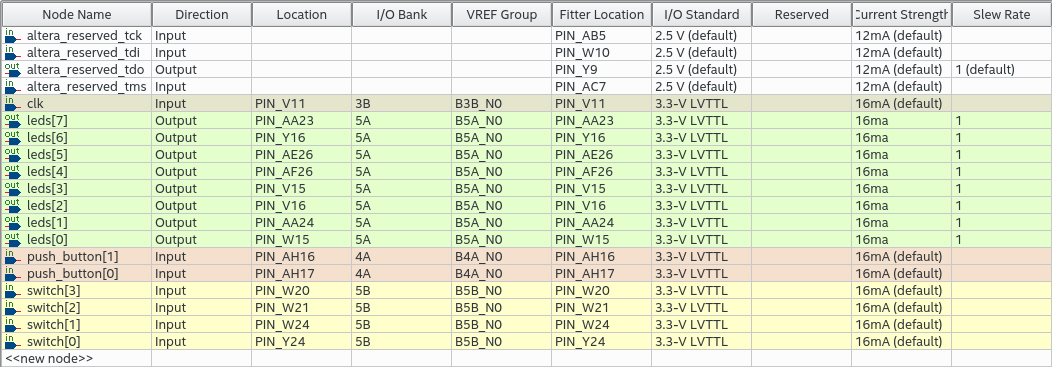
\includegraphics[scale=0.600]{12-pin-planner}
\caption{Pin Assignments in Pin Planner}
\label{fig:12-pin-planner}
\end{figure}

\item Update the timing constraints in \textbf{blink.sdc} to match the newly declared ports by replacing the contents of \textbf{blink.sdc} with the below code.
\newline
\newline
%Extract PDF Attachment: \textattachfile[
%	color=0.0 0.678 0.937,
%	mimetype=text/plain,
%	description={SDC Source File: blink.sdc}
%]{../../hdl_src/blink.sdc}{\textbf{blink.sdc}}
Download the blink.sdc file \href{\TheRawURL/MyFirstQsysSystem/hdl_src/blink.sdc}{\underline{here}}.
\newline
If you wish to view the blink.sdc file in the GitHub repo you can look \href{\TheBlobURL/MyFirstQsysSystem/hdl_src/blink.sdc}{\underline{here}}.

\inputminted[
	bgcolor=MyMintedBGColor,
	linenos,
	fontsize=\footnotesize
]{tcl}{../../hdl_src/blink.sdc}

\item Click the \textbf{Start Compilation} button in the top toolbar to compile the entire design.

\begin{figure}[H]
\centering
% screen shots report a density of 37.8 PixelsPerCentimeter when actual resolution
% is more like 56 PixelsPerCentimeter, so the scaling factor for 1:1 is 0.675
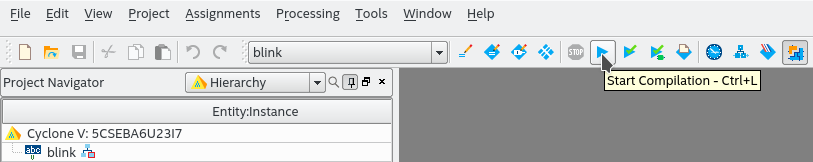
\includegraphics[scale=0.675]{14-start-compilation}
\caption{Start Compilation Button on Intel Quartus Software Toolbar}
\label{fig:14-start-compilation}
\end{figure}

\item After your design has successfully compiled, we will perform one last activity in the Intel Quartus software to prepare for the next tutorial that will actually make use of this system on the Terasic DE10-Nano board.  Since we have defined a memory mapped embedded system in Qsys with a JTAG master connected to a number of slave peripherals, it will be necessary for us to know what the base addresses are of the slave peripherals so we can interact with them, performing read and write transactions to them.  That base address information is captured in Qsys. You can visualize them in Qsys a number of ways, but that is not convenient for software developers or other users of this system to write code for it.  Each time you generate a Qsys system, Qsys outputs a database file called \textbf{<your-system-name>.sopcinfo}.  The Intel Quartus software tools installation provides a utility that can be used to translate the SOPCINFO database information into a usable macro format that can be used for various purposes called \textbf{sopc-create-header-files}.  The default functionality of \textbf{sopc-\allowbreak create-\allowbreak header-\allowbreak files} is to create C style header macros from each masters' perspective in the Qsys system.  We will perform this operation in the Intel Quartus software TCL Console which is located in the lower middle of the default Intel Quartus software GUI.  If you do not see the TCL Console pane, you can open it by selecting the \textbf{View} > \textbf{Utility Windows} > \textbf{TCL Console} menu.

\begin{figure}[H]
\centering
% screen shots report a density of 37.8 PixelsPerCentimeter when actual resolution
% is more like 56 PixelsPerCentimeter, so the scaling factor for 1:1 is 0.675
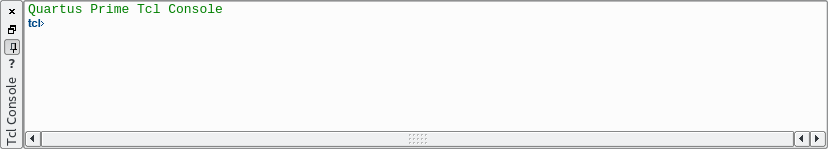
\includegraphics[scale=0.675]{15-tcl-console}
\caption{Intel Quartus Prime Software TCL Console}
\label{fig:15-tcl-console}
\end{figure}

We will first create a directory to output the header files into, then we will create the default header file output using \textbf{sopc-create-header-files} and finally we will extract the base address entries out of the JTAG master header file for the FPGA peripherals that it is connected to.  We will perform all of this with the following TCL commands:

\begin{minted}[
	fontsize=\footnotesize,
	bgcolor=MyMintedBGColor,
	escapeinside=++
]{text}

Quartus Prime Tcl Console

# make a directory called 'qsys_headers' to store the header files
tcl> file mkdir qsys_headers

# create a TCL variable SCHF_PATH to hold the path to the executable program
# sopc-create-header-files on your host PC using the environment variables
# provided by Quartus.
tcl> set SCHF_PATH [glob -join +\$+quartus(quartus_rootpath) sopc_builder bin sopc-create-header-files]

# create a TCL variable BAT_PATH to hold the path to the Nios II Command Shell
# batch file on Windows platforms.  The following code sequence will work on
# either Windows or Linux.  For Linux this variable will just be set to NULL.
tcl> set BAT_PATH {}
tcl> if {+\$+tcl_platform(platform) == "windows"} {
   > set BAT_PATH [glob -join +\$+quartus(quartus_rootpath) .. nios2eds {Nios II Command Shell.bat}]
   > }

# execute sopc-create-header-files to generate the header files
tcl> eval exec -ignorestderr +\$+{BAT_PATH} +\$+{SCHF_PATH} soc_system.sopcinfo --output-dir qsys_headers

# read the header file for master_0 into a TCL variable
tcl> set master_0_header [read [open [glob -join qsys_headers master_0.h] r]]

# output the C macro lines for the FPGA peripheral base addresses
tcl> foreach line [split +\$+{master_0_header} "\n"] { \
   > if {[string match "*_BASE*" +\$+{line}]} {puts +\$+{line}}}

\end{minted}

If you have put your Qsys system together properly and executed the above commands correctly, you should see the following output in the Intel Quartus software TCL console representing the base address definitions for the five Qsys peripherals in the FPGA fabric connected to master\_0, the JTAG master bridge component.

\begin{minted}[
	bgcolor=MyMintedBGColor,
	escapeinside=++
]{c}

#define OCRAM_64K_BASE 0x0
#define LED_PIO_BASE 0x10000
#define BUTTON_PIO_BASE 0x10010
#define SWITCH_PIO_BASE 0x10020
#define SYSTEM_ID_BASE 0x10030

\end{minted}

\end{enumerate}

That's it! You have designed and compiled your first Qsys system.  This basic design is intended as a stepping stone to the next tutorials and it won't do much on its own when programmed into your device. Continue to the \textquote{Interacting with FPGA Designs Using System Console} tutorial where we demonstrate how to use the System Console tool to program the FPGA and interact with this design.

\end{flushleft}

\end{document}

